%%% Local Variables:
%%% mode: latex; mode: flyspell
%%% TeX-master: "."
%%% End:

\section { Fits }
The published data was fit using both of the published response functions.
The method to fit the data was to minimize the $\chi^2$ value for many values
of kMax, and then fit a parabola to the $\chi^2$ distribution, 
$\chi^2_{Min} + \frac{(k-kMax)^2}{\sigma^2}$. The uncertainty on the fit kMax
is then the inverse square root of the coefficient. This was also done using
a negative log likelihood (NLL) minimization strategy, where the variance is half of
the inverse of the leading coefficient. The latter is able to take into account empty
bins in the data while the former cannot. The end point values for each target z 
are shown in figure \ref{fig:ChiSq} and \ref{fig:NLL} using $\chi^2$ and NLL minimization
respectively, and the $\chi^2$/DoF is shown in figure \ref{fig:ChiSqOfFits}. The NLL
fitting method includes empty bins, which are ignored by the $\chi^2$ fitting method,
and has a greater cost for deviating from bins with small entry numbers. This results
in the NLL fit end point values being consistently higher, as is shown in figure \ref{fig:compareFits}.

\begin{figure}[h]
  \centering
  \subfloat[ $\chi^2$ Minimization Fit \label{fig:ChiSq}]{%
  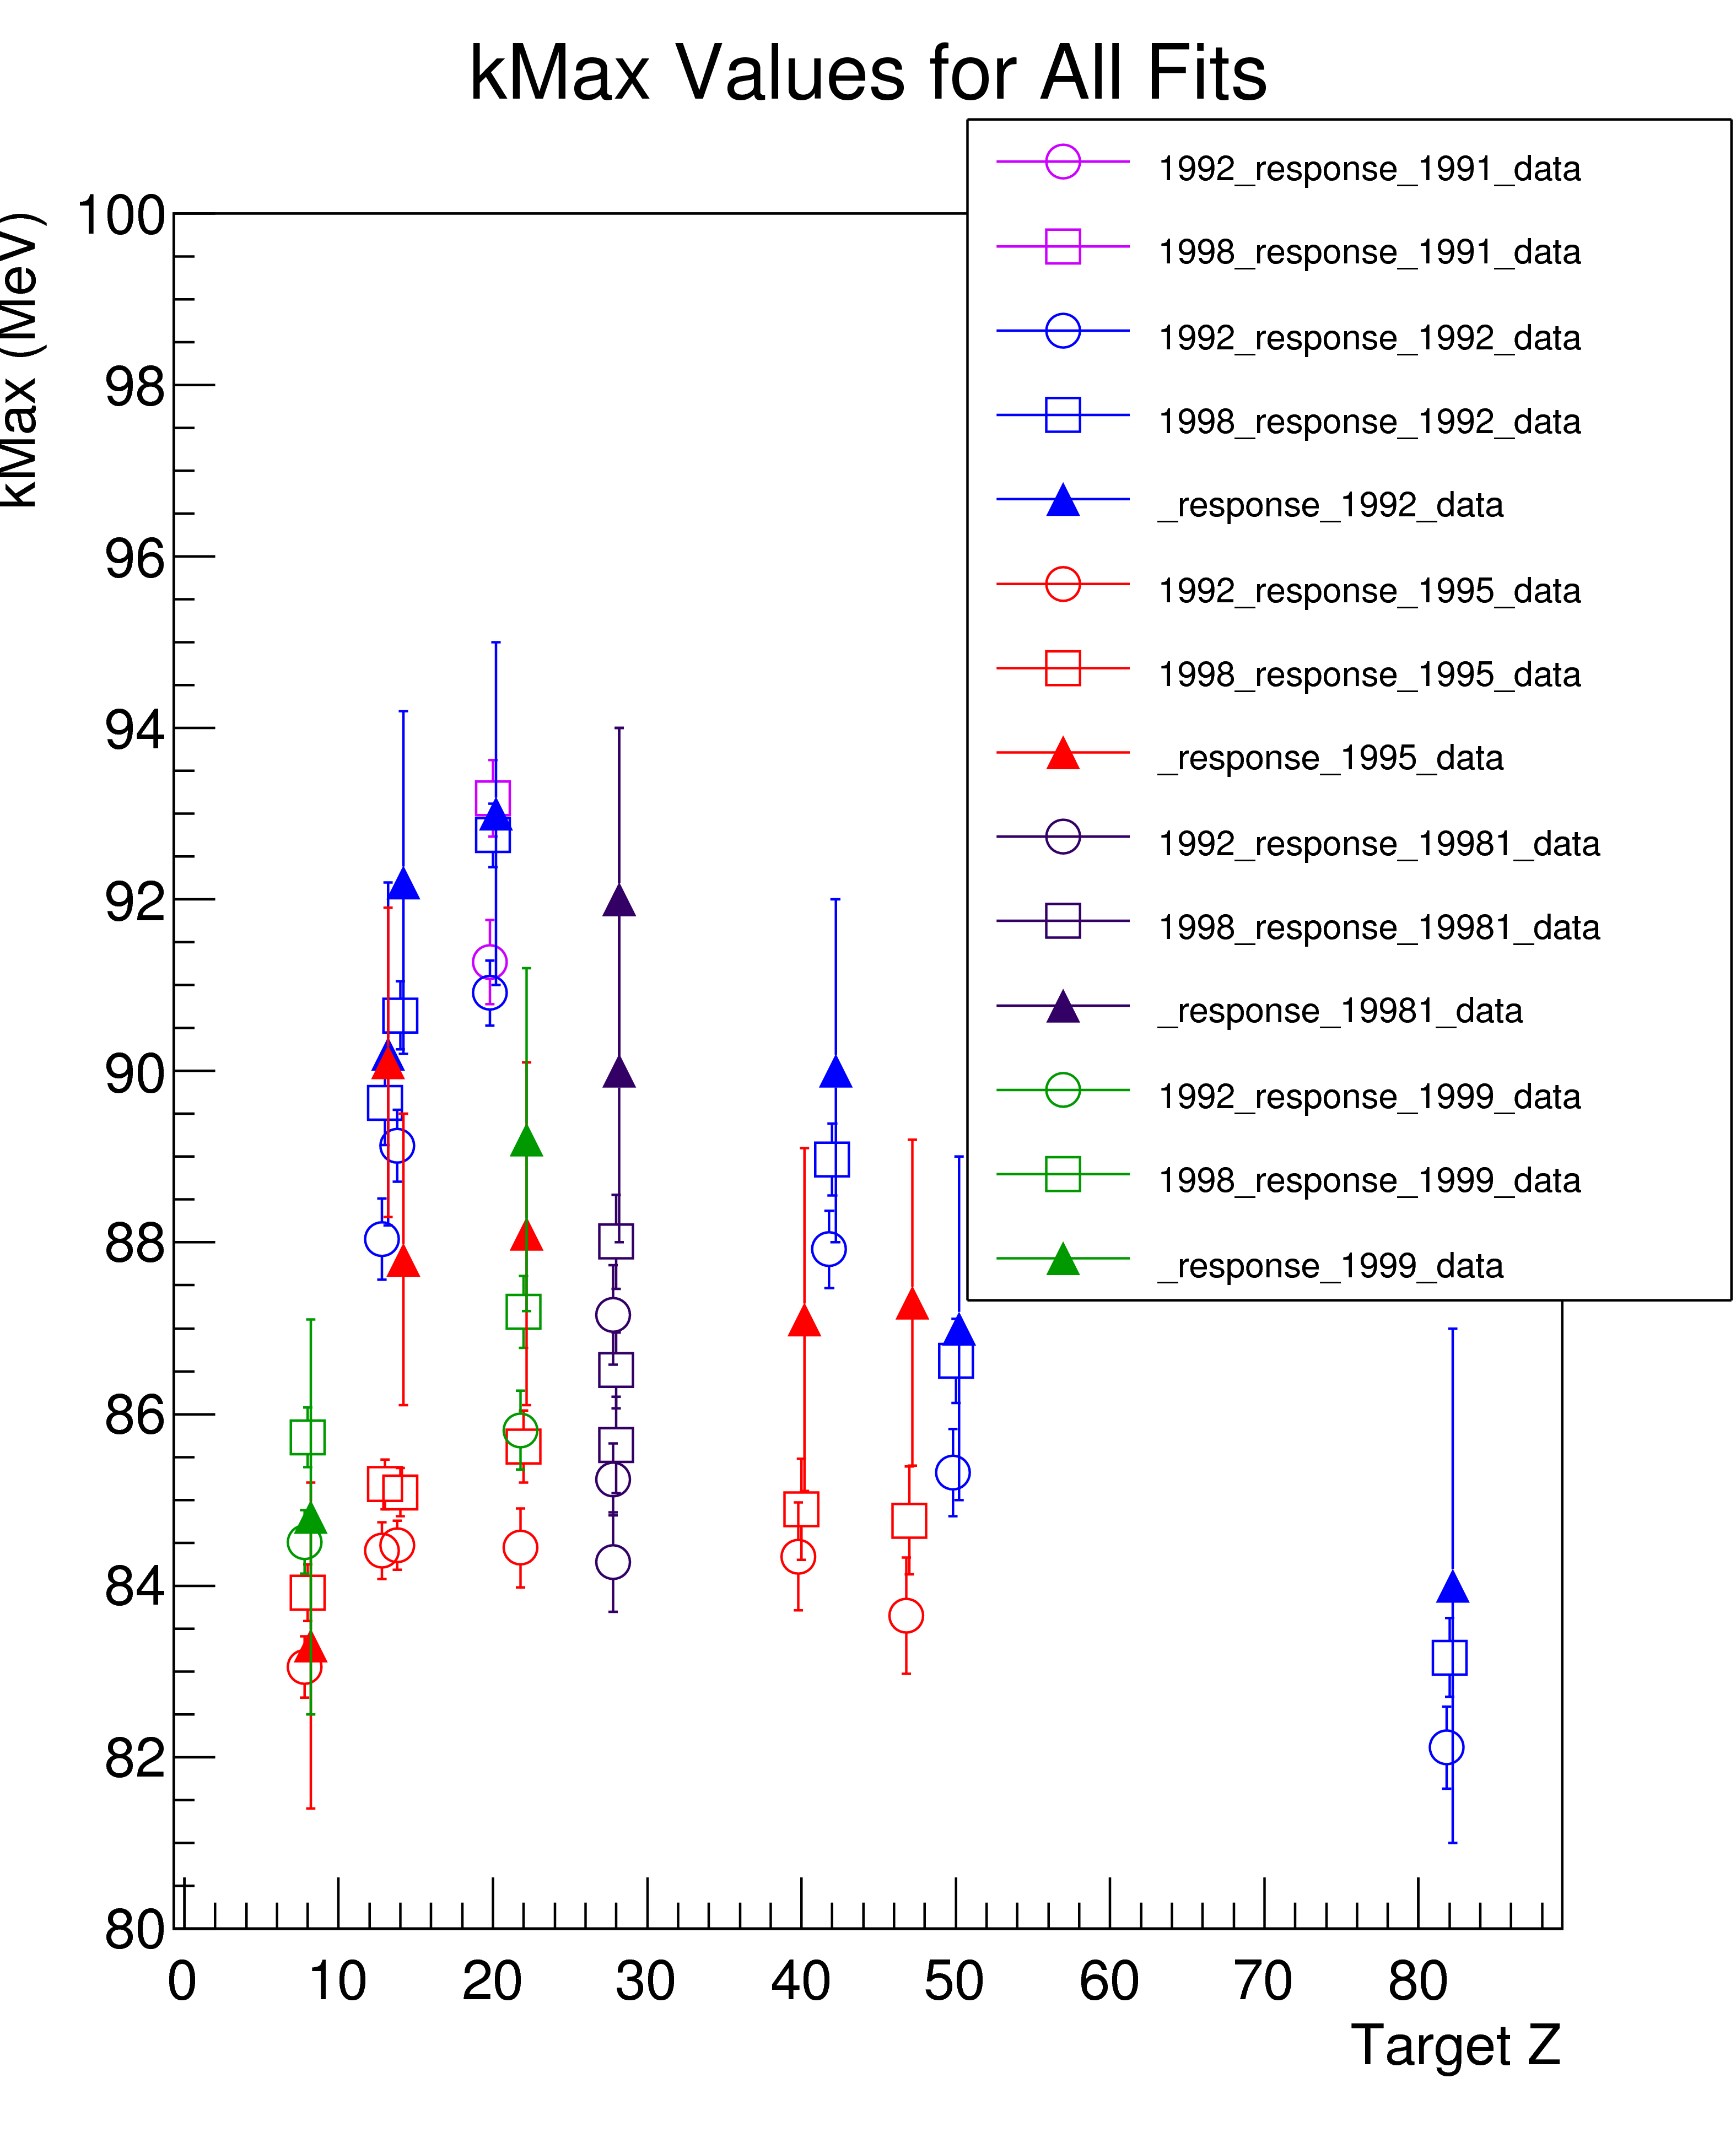
\includegraphics[width=0.48\linewidth]{figures/png/all_kMaxesChiSq_vs_target_z.png}
  }
  \hfill
  \subfloat[NLL Minimization Fit  \label{fig:NLL}]{%
  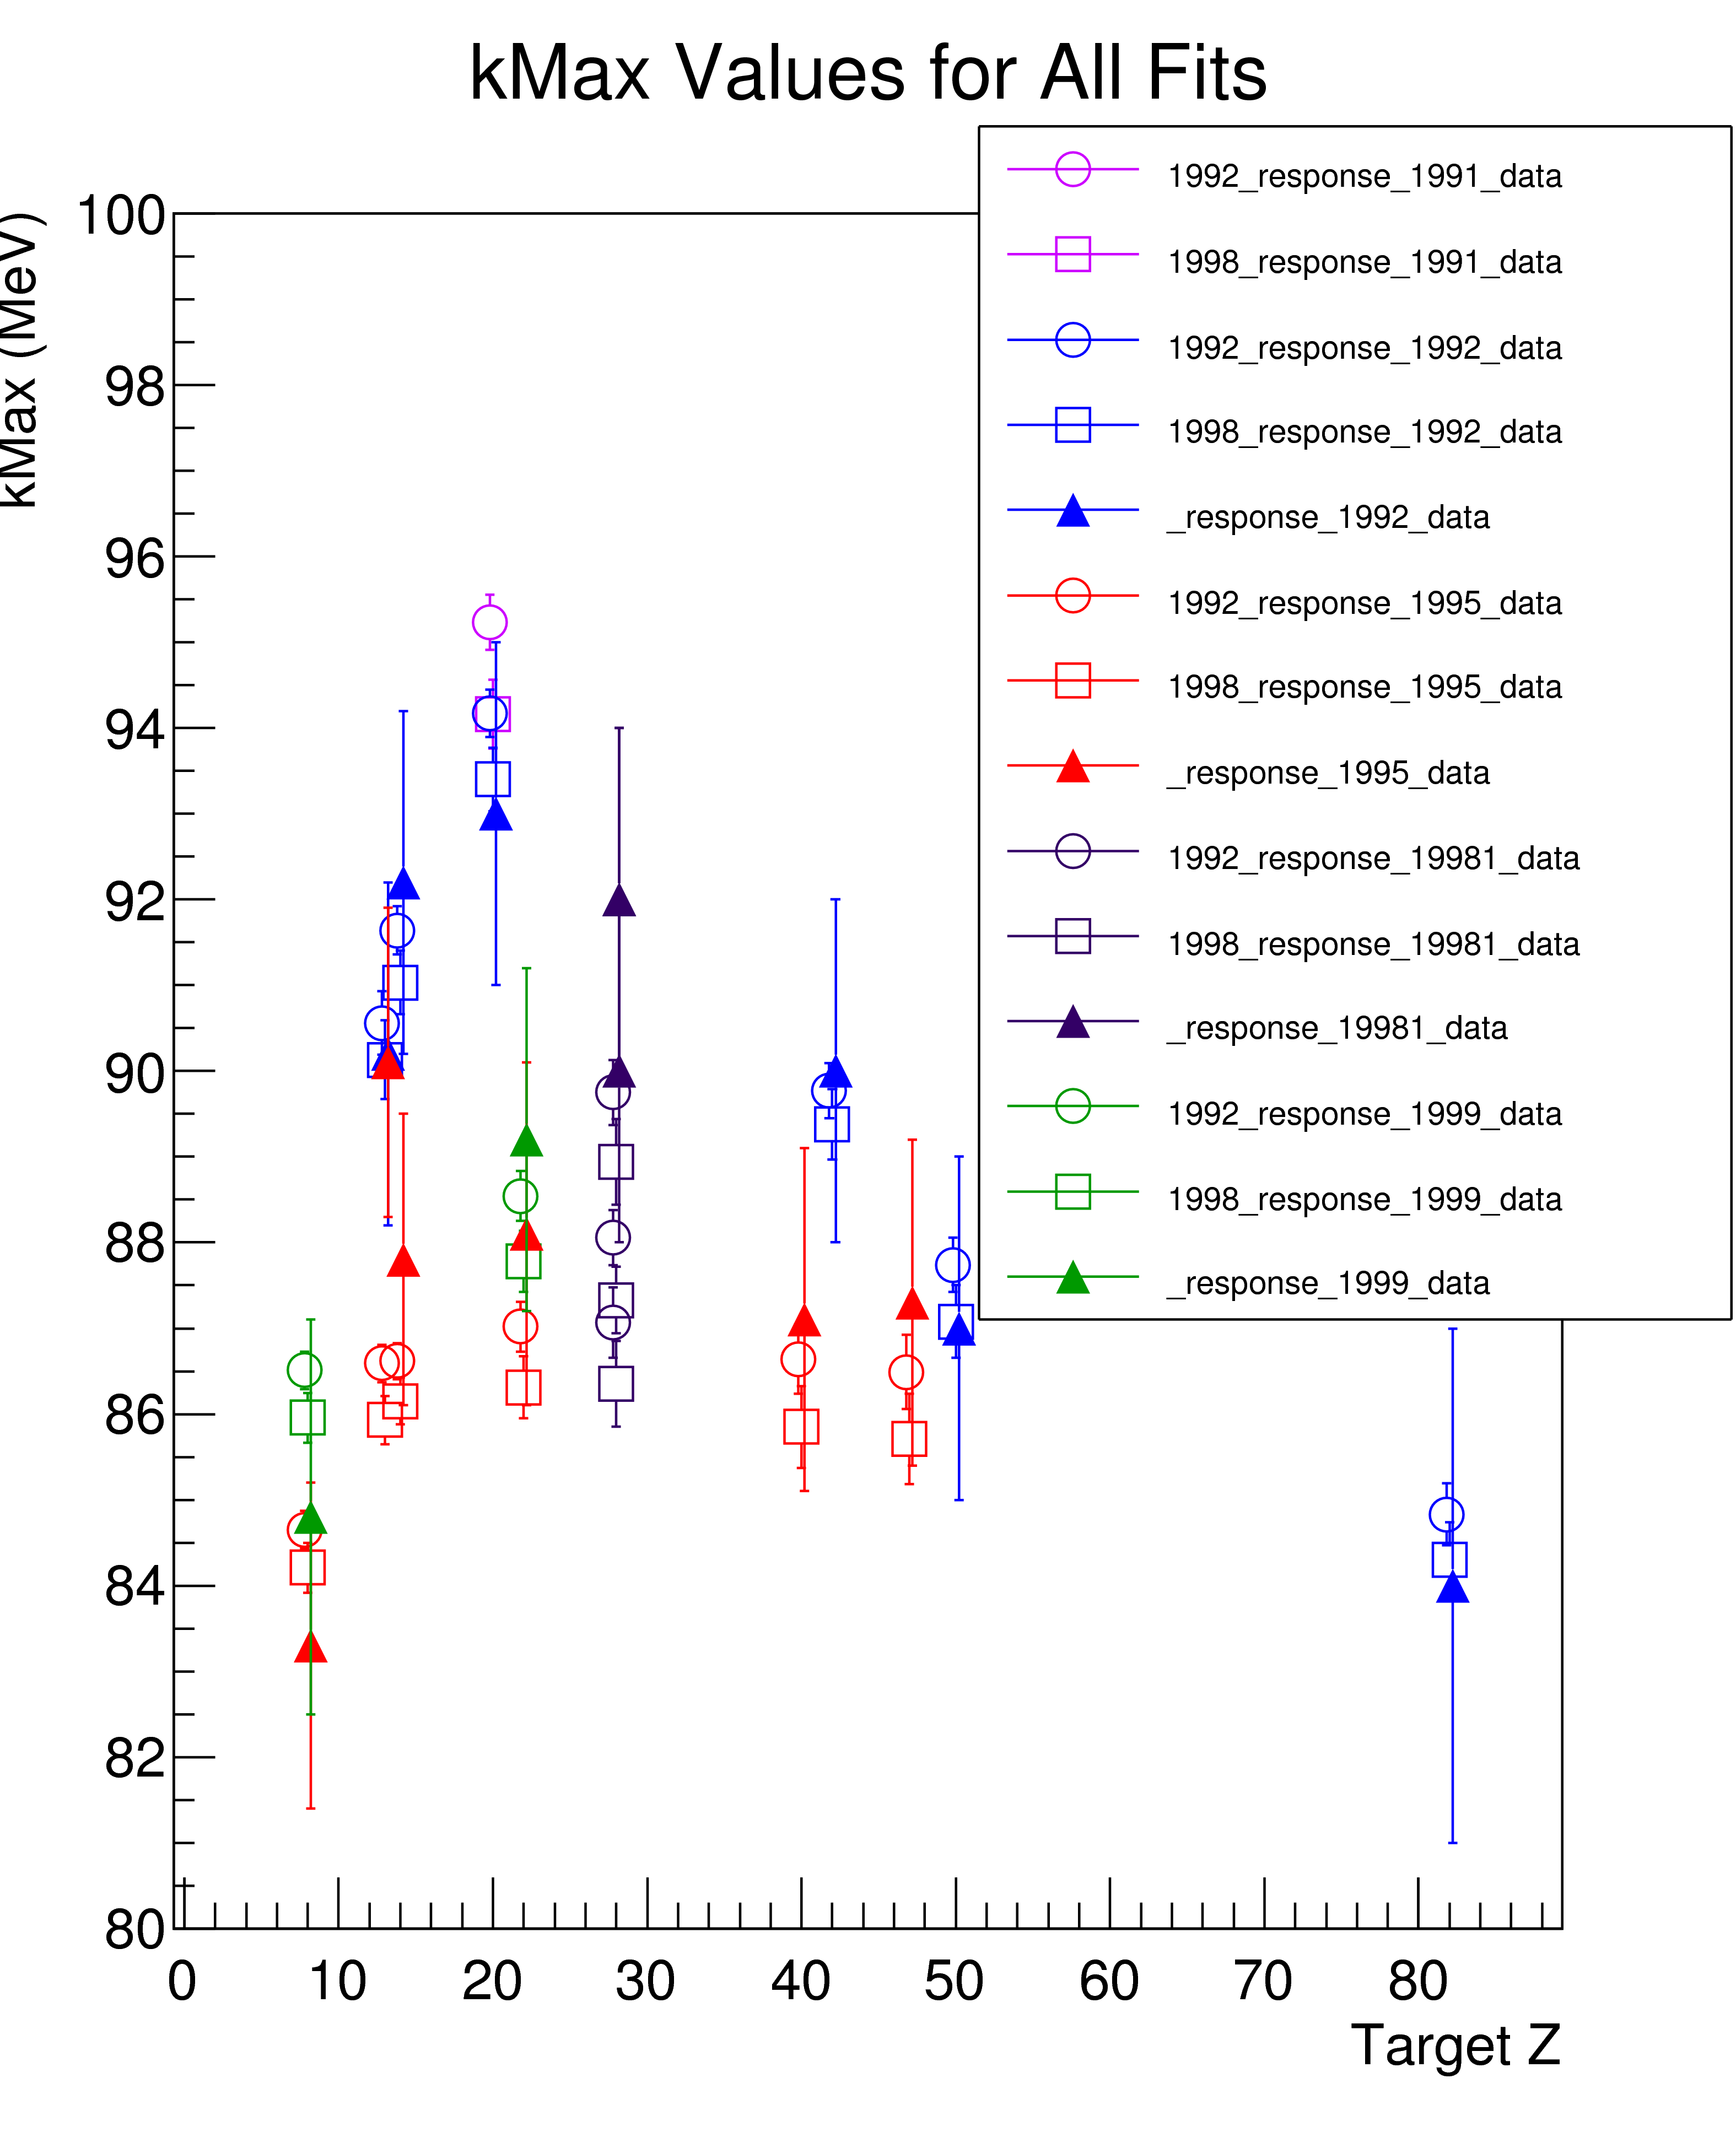
\includegraphics[width=0.48\linewidth]{figures/png/all_kMaxesNLL_vs_target_z.png}
  }
  \caption{Best fit end point value vs nuclear targets using (a) $\chi^2$ minimization and (b) NLL minimization.
    Triangular markers indicate the published values and uncertainty, circular markers indicate the results
    using the published 1992 response function, and square markers indicate the results using the published
    1998 response function. The 1992 response function data points are offset by -0.2 from their target z values
    and the published data points are offset by 0.2 from their target z values.
  }
\end{figure}
\begin{figure}[h]
  \centering
  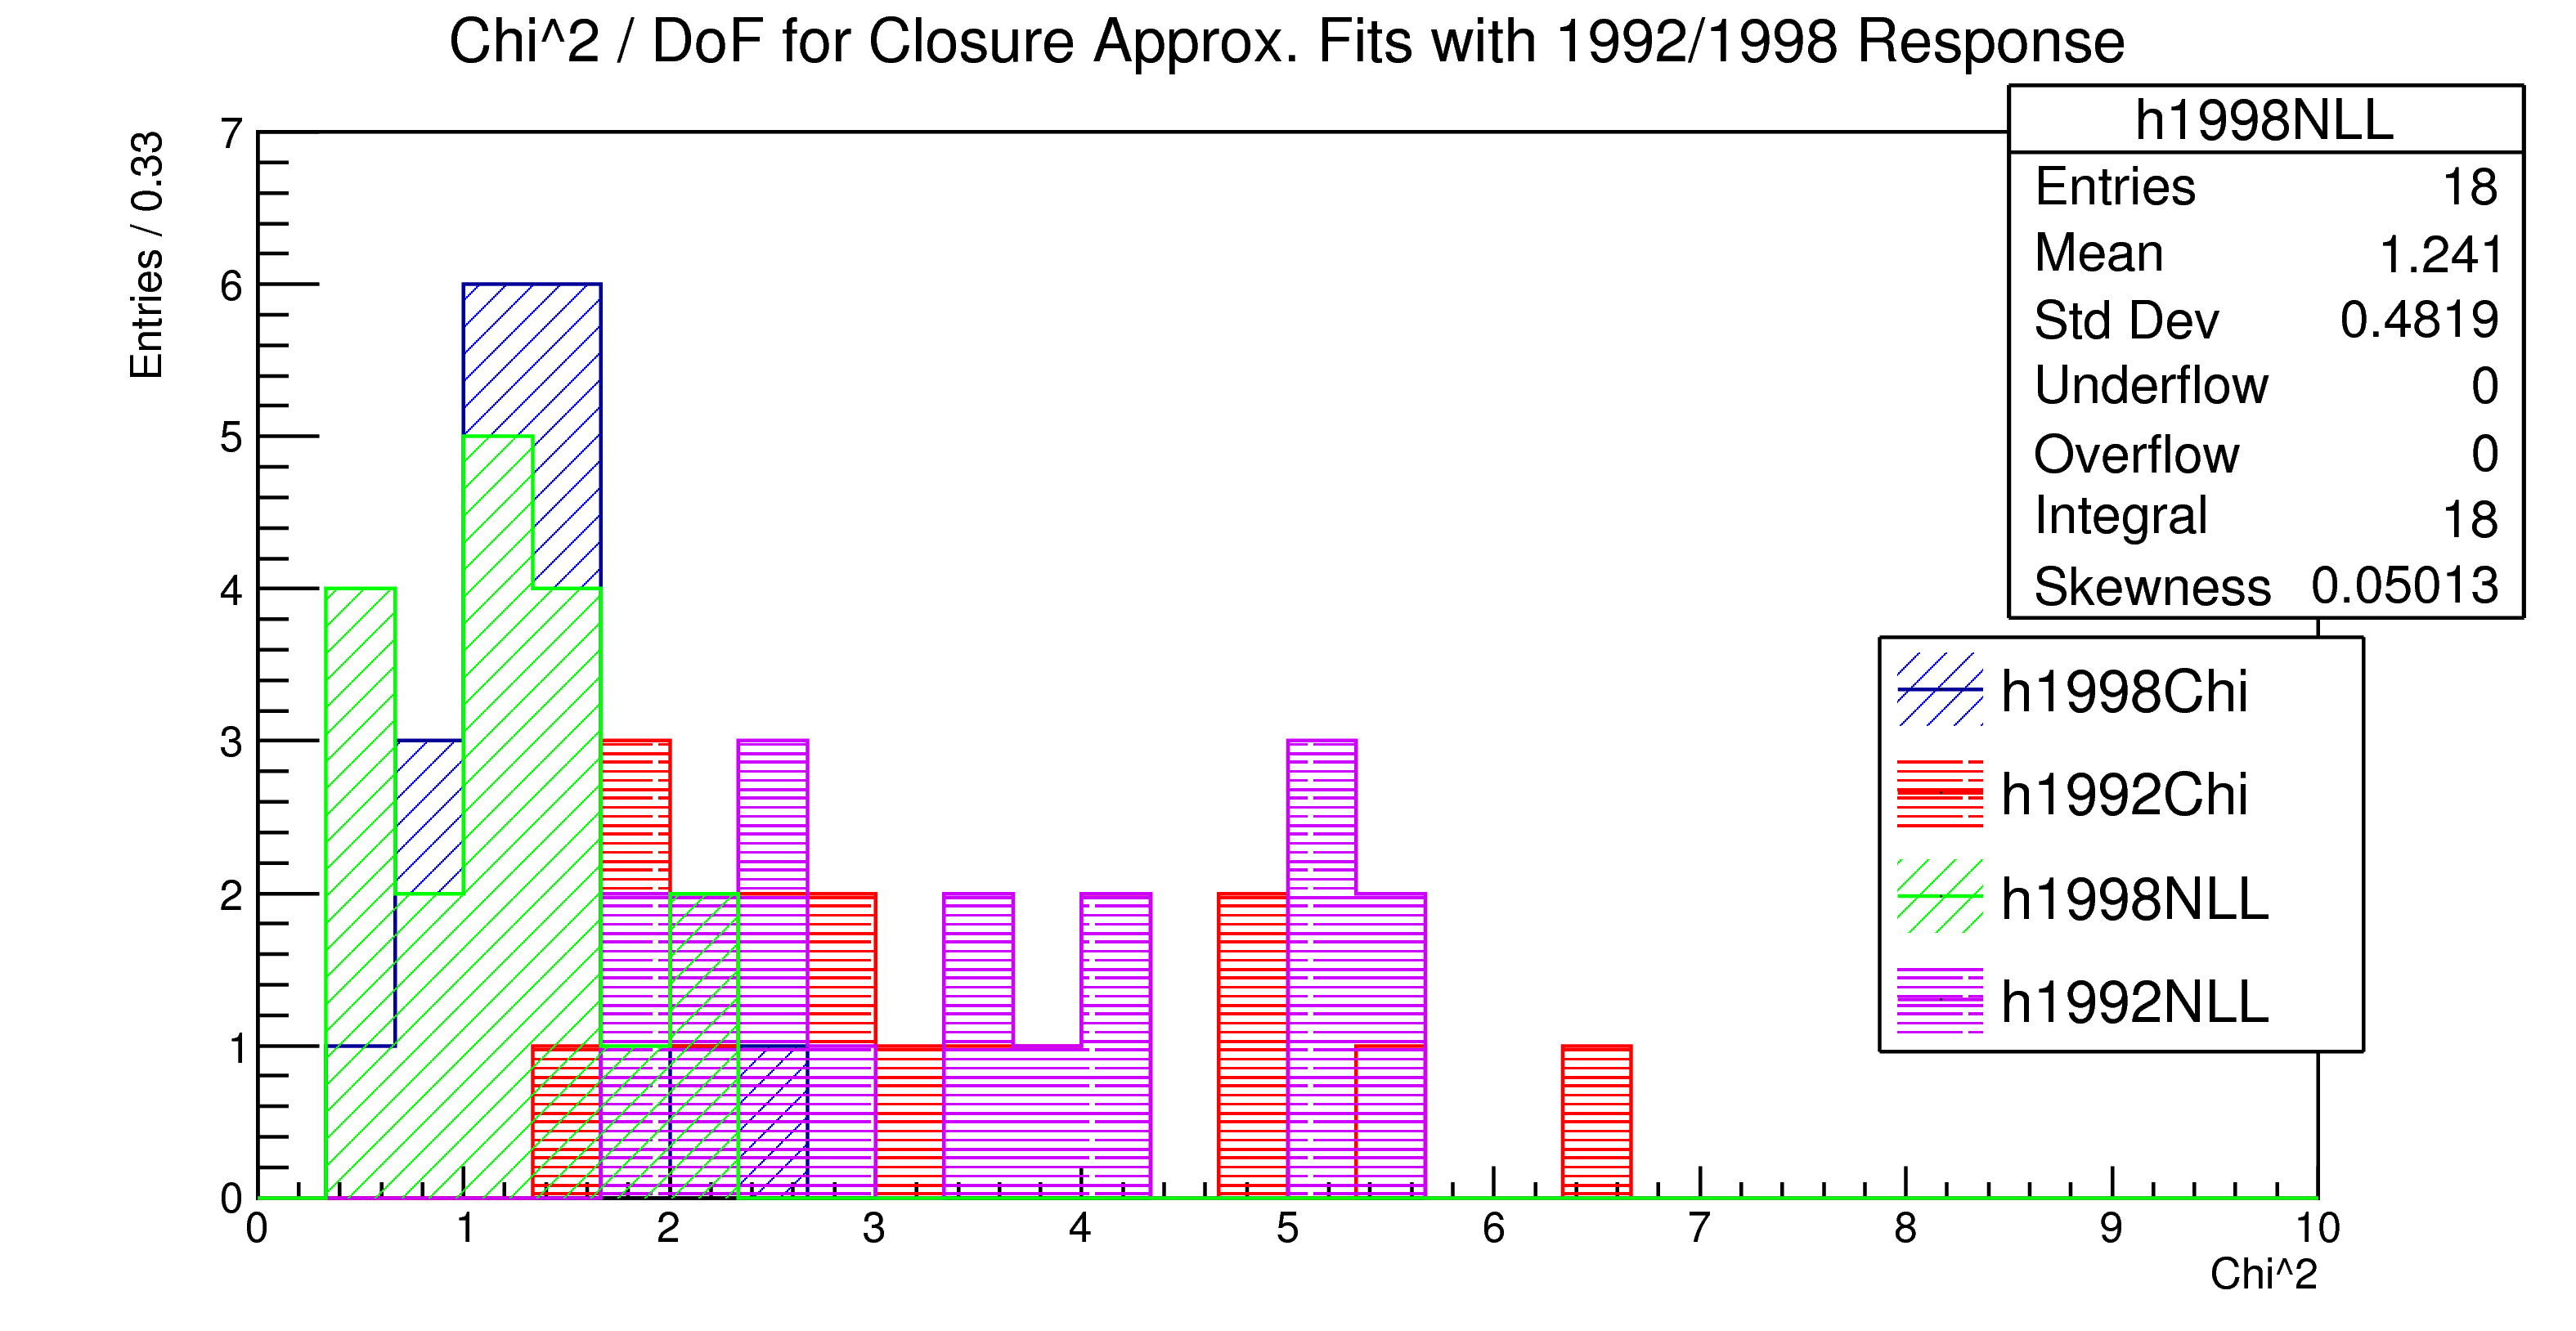
\includegraphics[width=0.8\linewidth]{figures/png/chiSq_of_fits.png}
  \caption{Fit $\chi^2$ values for both response functions and both fitting methods. }
  \label{fig:ChiSqOfFits}
\end{figure}



%%%%%%%%%%%%%%%%%%%%%%%%%%%%%%%%%%%%%%%%%%%%%%%%%%%%%%%%%%%%%%%%%%%%%%%%%%%%%%

\subsection { Fits of the 1992 data }
\begin{table}[H]
  \begin{center}
    \begin{tabular}{|l||l|l|l|l|l|l|}
      \hline
      Dataset & Published $k_{Max}$ & $\chi^2 / DoF$ & Our $k_{Max}$ & $\chi^2 / DoF$  & Response & Fit \\
      \hhline{|=||=|=|=|=|=|=|}
       Al 1992   & 90.2 $\pm$ 2   & 1.1 & 88.0 $\pm$ 0.5 & 1.7 (57.2 / 34) & 1992 & $\chi^2$ \\  
                 &                &     & 89.6 $\pm$ 0.5 & 1.0 (33.9 / 34) & 1998 & $\chi^2$ \\  
                                                                            
                 &                &     & 90.6 $\pm$ 0.4 & 2.3 (98.1 / 43) & 1992 & NLL \\
                 &                &     & 90.1 $\pm$ 0.5 & 1.3 (54.3 / 43) & 1998 & NLL \\
       \hline                                                               
       Ca 1992   & 93   $\pm$ 2   & 1.6 & 90.9 $\pm$ 0.4 & 2.9 (113.4 / 39)& 1992 & $\chi^2$ \\  
                 &                &     & 92.8 $\pm$ 0.4 & 1.2 (48.4 / 39) & 1998 & $\chi^2$ \\  
                                                                            
                 &                &     & 94.2 $\pm$ 0.3 & 4.8 (205.0 / 43)& 1992 & NLL \\
                 &                &     & 93.4 $\pm$ 0.4 & 1.6 (68.3 / 43) & 1998 & NLL \\
      \hline                                                                
       Mo 1992   & 90   $\pm$ 2   & 0.8 & 87.9 $\pm$ 0.5 & 1.8 (58.0 / 32) & 1992 & $\chi^2$ \\  
                 &                &     & 89.0 $\pm$ 0.4 & 0.7 (22.4 / 32) & 1998 & $\chi^2$ \\  
                                                                            
                 &                &     & 89.8 $\pm$ 0.3 & 1.8 (77.2 / 43) & 1992 & NLL \\
                 &                &     & 89.4 $\pm$ 0.4 & 0.6 (27.1 / 43) & 1998 & NLL \\
      \hline                                                                
       Pb 1992   & 84   $\pm$ 3   & 0.9 & 82.1 $\pm$ 0.5 & 1.4 (43.9 / 31) & 1992 & $\chi^2$ \\  
                 &                &     & 83.2 $\pm$ 0.5 & 0.6 (17.6 / 31) & 1998 & $\chi^2$ \\  
                                                                            
                 &                &     & 84.8 $\pm$ 0.4 & 1.8 (79.5 / 43) & 1992 & NLL \\
                 &                &     & 84.3 $\pm$ 0.4 & 0.5 (22.3 / 43) & 1998 & NLL \\
      \hline                                                                
       Si 1992   & 92.2 $\pm$ 2   & 1.7 & 89.1 $\pm$ 0.4 & 3.5 (116.9 / 33)& 1992 & $\chi^2$ \\  
                 &                &     & 90.6 $\pm$ 0.4 & 1.3 (43.4 / 33) & 1998 & $\chi^2$ \\  
                                                                            
                 &                &     & 91.6 $\pm$ 0.3 & 3.7 (160.2 / 43)& 1992 & NLL \\
                 &                &     & 91.0 $\pm$ 0.4 & 1.3 (54.1 / 43) & 1998 & NLL \\
      \hline                                                                
       Sn 1992   & 87   $\pm$ 2   & 1.1 & 85.3 $\pm$ 0.5 & 2.6 (79.6 / 31) & 1992 & $\chi^2$ \\  
                 &                &     & 86.6 $\pm$ 0.5 & 0.7 (22.1 / 31) & 1998 & $\chi^2$ \\  
                                                                            
                 &                &     & 87.7 $\pm$ 0.3 & 2.5 (105.8 / 43) & 1992 & NLL \\
                 &                &     & 87.1 $\pm$ 0.4 & 0.6 (24.1 / 43) & 1998 & NLL \\
      \hline                           
    \end{tabular}
  \end{center}
  \caption{The fit results.}
  \label{table:fits1992}
\end{table}

%%%%%%%%%%%%%%%%%%%%%%%%%%%%%%%%%%%%%%%%%%%%%%%%%%%%%%%%%%%%%%%%%%%%%%%%%%%%%%
\subsection { Fits of the 1995 data }

\begin{table}[H]
  \begin{center}
    \begin{tabular}{|l||l|l|l|l|l|l|}
      \hline
      Dataset & Published $k_{Max}$ & $\chi^2 / DoF$ & Our $k_{Max}$ & $\chi^2 / DoF$  & Response & Fit \\
      \hhline{|=||=|=|=|=|=|=|}
       Ag 1995   & 87.3 $\pm$ 1.9 & 1.0 &83.7 $\pm$ 0.7 & 2.2 (64.8 / 30)  & 1992 & $\chi^2$ \\  
                 &                &     &84.8 $\pm$ 0.6 & 1.0 (30.3 / 30)  & 1998 & $\chi^2$ \\  
                                                                            
                &                &     & 86.5 $\pm$ 0.4 & 2.1 (91.8 / 43) & 1992 & NLL \\
                &                &     & 85.7 $\pm$ 0.5 & 0.8 (36.1 / 43) & 1998 & NLL \\      
      \hline                                                               
       Al 1995   & 90.1 $\pm$ 1.8 & 1.6 &84.4 $\pm$ 0.3 & 4.8 (153.2 / 32) & 1992 & $\chi^2$ \\  
                 &                &     &85.2 $\pm$ 0.3 & 1.4 (46.4 / 32)  & 1998 & $\chi^2$ \\  
                                                                           
                &                &     & 86.6 $\pm$ 0.2 & 4.8 (205.2 / 43) & 1992 & NLL \\
                &                &     & 85.9 $\pm$ 0.3 & 1.3 (56.3 / 43) & 1998 & NLL \\
      \hline                                                               
       O 1995    & 87.1 $\pm$ 1.9 & 1.5 &83.0 $\pm$ 0.4 & 5.0 (123.9 / 25) & 1992 & $\chi^2$ \\  
                 &                &     &83.9 $\pm$ 0.3 & 1.4 (34.0 / 25)  & 1998 & $\chi^2$ \\  
                                                                           
                &                &     & 84.6 $\pm$ 0.2 & 3.5 (149.5 / 43)& 1992 & NLL\\
                &                &     & 84.2 $\pm$ 0.3 & 1.1 (49.2 / 43) & 1998 & NLL\\
      \hline                                                                    
       Si 1995   & 87.8 $\pm$ 1.7 & 1.9 &84.5 $\pm$ 0.3 & 5.4 (168.3 / 31) & 1992 & $\chi^2$ \\  
                 &                &     &85.1 $\pm$ 0.3 & 2.4 (74.7 / 31)  & 1998 & $\chi^2$ \\  
                                                                            
                &                &     & 86.6 $\pm$ 0.2 & 5.3 (227.9 / 43) & 1992 & NLL \\
                &                &     & 86.1 $\pm$ 0.3 & 2.1 (88.9 / 43) & 1998 & NLL \\
      \hline                                                               
       Ti 1995   & 88.1 $\pm$ 2.0 & 1.5 &84.4 $\pm$ 0.5 & 3.9 (124.1 / 32) & 1992 & $\chi^2$ \\  
                 &                &     &85.6 $\pm$ 0.4 & 1.5 (48.7 / 32)  & 1998 & $\chi^2$ \\  
                                                                           
                &                &     & 87.0 $\pm$ 0.3 & 3.9 (169.0 / 43) & 1992 & NLL \\
                &                &     & 86.3 $\pm$ 0.4 & 1.3 (56.8 / 43) & 1998 & NLL \\
      \hline                                                               
       Zr 1995   & 87.1 $\pm$ 2.0 & 1.3 &84.3 $\pm$ 0.6 & 3.1 (94.9 / 31)  & 1992 & $\chi^2$ \\  
                 &                &     &84.9 $\pm$ 0.6 & 1.6 (51.1 / 31)  & 1998 & $\chi^2$ \\  
                                                                           
                &                &     & 86.6 $\pm$ 0.4 & 2.8 (119.4 / 43) & 1992 & NLL \\
                &                &     & 85.9 $\pm$ 0.5 & 1.4 (59.3 / 43) & 1998 & NLL \\
      \hline
                                                                                
    \end{tabular}
  \end{center}
  \caption{The fit results.}
  \label{table:fits1995}
\end{table}

%%%%%%%%%%%%%%%%%%%%%%%%%%%%%%%%%%%%%%%%%%%%%%%%%%%%%%%%%%%%%%%%%%%%%%%%%%%%%%
\subsection { Fits of the 1998 data }
\begin{table}[H]
  \begin{center}
    \begin{tabular}{|l||l|l|l|l|l|l|}
      \hline
      Dataset & Published $k_{Max}$ & $\chi^2 / DoF$ & Our $k_{Max}$ & $\chi^2 / DoF$  & Response & Fit \\
      \hhline{|=||=|=|=|=|=|=|}
       Ni58 1998 & 92   $\pm$ 2   & 1.8 & 87.2 $\pm$ 0.6 & 2.5 (80.6 / 32) & 1992 & $\chi^2$ \\  
                 &                &     & 88.0 $\pm$ 0.5 & 1.1 (35.6 / 32) & 1998 & $\chi^2$ \\  
                                                                            
                &                 &     & 89.7 $\pm$ 0.4 & 2.5 (106.8 / 43) & 1992 & NLL \\
                &                 &     & 88.9 $\pm$ 0.5 & 1.0 (41.2 / 43) & 1998 & NLL \\
      \hline                                                                
       Ni60 1998 & 92   $\pm$ 2   & 2.0 & 85.2 $\pm$ 0.4 & 2.7 (90.3 / 33) & 1992 & $\chi^2$ \\  
                 &                &     & 86.5 $\pm$ 0.4 & 1.1 (37.0 / 33) & 1998 & $\chi^2$ \\  
                                                                            
                &                 &     & 88.1 $\pm$ 0.3 & 3.3 (143.5 / 43) & 1992 & NLL \\
                &                 &     & 87.3 $\pm$ 0.4 & 1.0 (41.5 / 43) & 1998 & NLL \\
      \hline                                                                
       Ni62 1998 & 90   $\pm$ 2   & 1.3 & 84.3 $\pm$ 0.6 & 1.8 (52.6 / 30) & 1992 & $\chi^2$ \\  
                 &                &     & 85.6 $\pm$ 0.6 & 0.8 (24.1 / 30) & 1998 & $\chi^2$ \\  
                                                                            
                &                 &     & 87.1 $\pm$ 0.4 & 1.9 (79.9 / 43) & 1992 & NLL \\
                &                 &     & 86.3 $\pm$ 0.5 & 0.6 (25.8 / 43) & 1998 & NLL \\
      \hline                           
    \end{tabular}
  \end{center}
  \caption{The fit results.}
  \label{table:fits1998}
\end{table}

%%%%%%%%%%%%%%%%%%%%%%%%%%%%%%%%%%%%%%%%%%%%%%%%%%%%%%%%%%%%%%%%%%%%%%%%%%%%%%
\subsection { Fits of the 1999 data }

\begin{table}[H]
  \begin{center}
    \begin{tabular}{|l||l|l|l|l|l|l|}
      \hline
      Dataset & Published $k_{Max}$ & $\chi^2 / DoF$ & Our $k_{Max}$ & $\chi^2 / DoF$  & Response & Fit \\
      \hhline{|=||=|=|=|=|=|=|}
       O 1999    & 88.4 $\pm$ 2.3 & 2.1 & 84.5 $\pm$ 0.4 & 6.4 (178.3 / 28)& 1992 & $\chi^2$ \\  
                 &                &     & 85.7 $\pm$ 0.4 & 2.0 (55.8 / 28) & 1998 & $\chi^2$ \\  
                                                                            
                 &                &     & 86.5 $\pm$ 0.2 & 4.9 (212.8 / 43)& 1992 & NLL\\
                 &                &     & 86.0 $\pm$ 0.3 & 2.1 (89.4 / 43) & 1998 & NLL\\
      \hline                                                                
       Ti 1999   & 89.2 $\pm$ 2.0 & 1.9 & 85.8 $\pm$ 0.5 & 4.1 (135.6 / 33)& 1992 & $\chi^2$ \\  
                 &                &     & 87.2 $\pm$ 0.4 & 1.6 (52.3 / 33) & 1998 & $\chi^2$ \\  
                                                                            
                 &                &     & 88.5 $\pm$ 0.3 & 4.2 (178.6 / 43) & 1992 & NLL \\
                 &                &     & 87.8 $\pm$ 0.4 & 1.2 (50.9 / 43) & 1998 & NLL \\
      \hline                           
    \end{tabular}
  \end{center}
  \caption{The fit results.}
  \label{table:fits1999}
\end{table}

\begin{figure}[h]
  \centering
  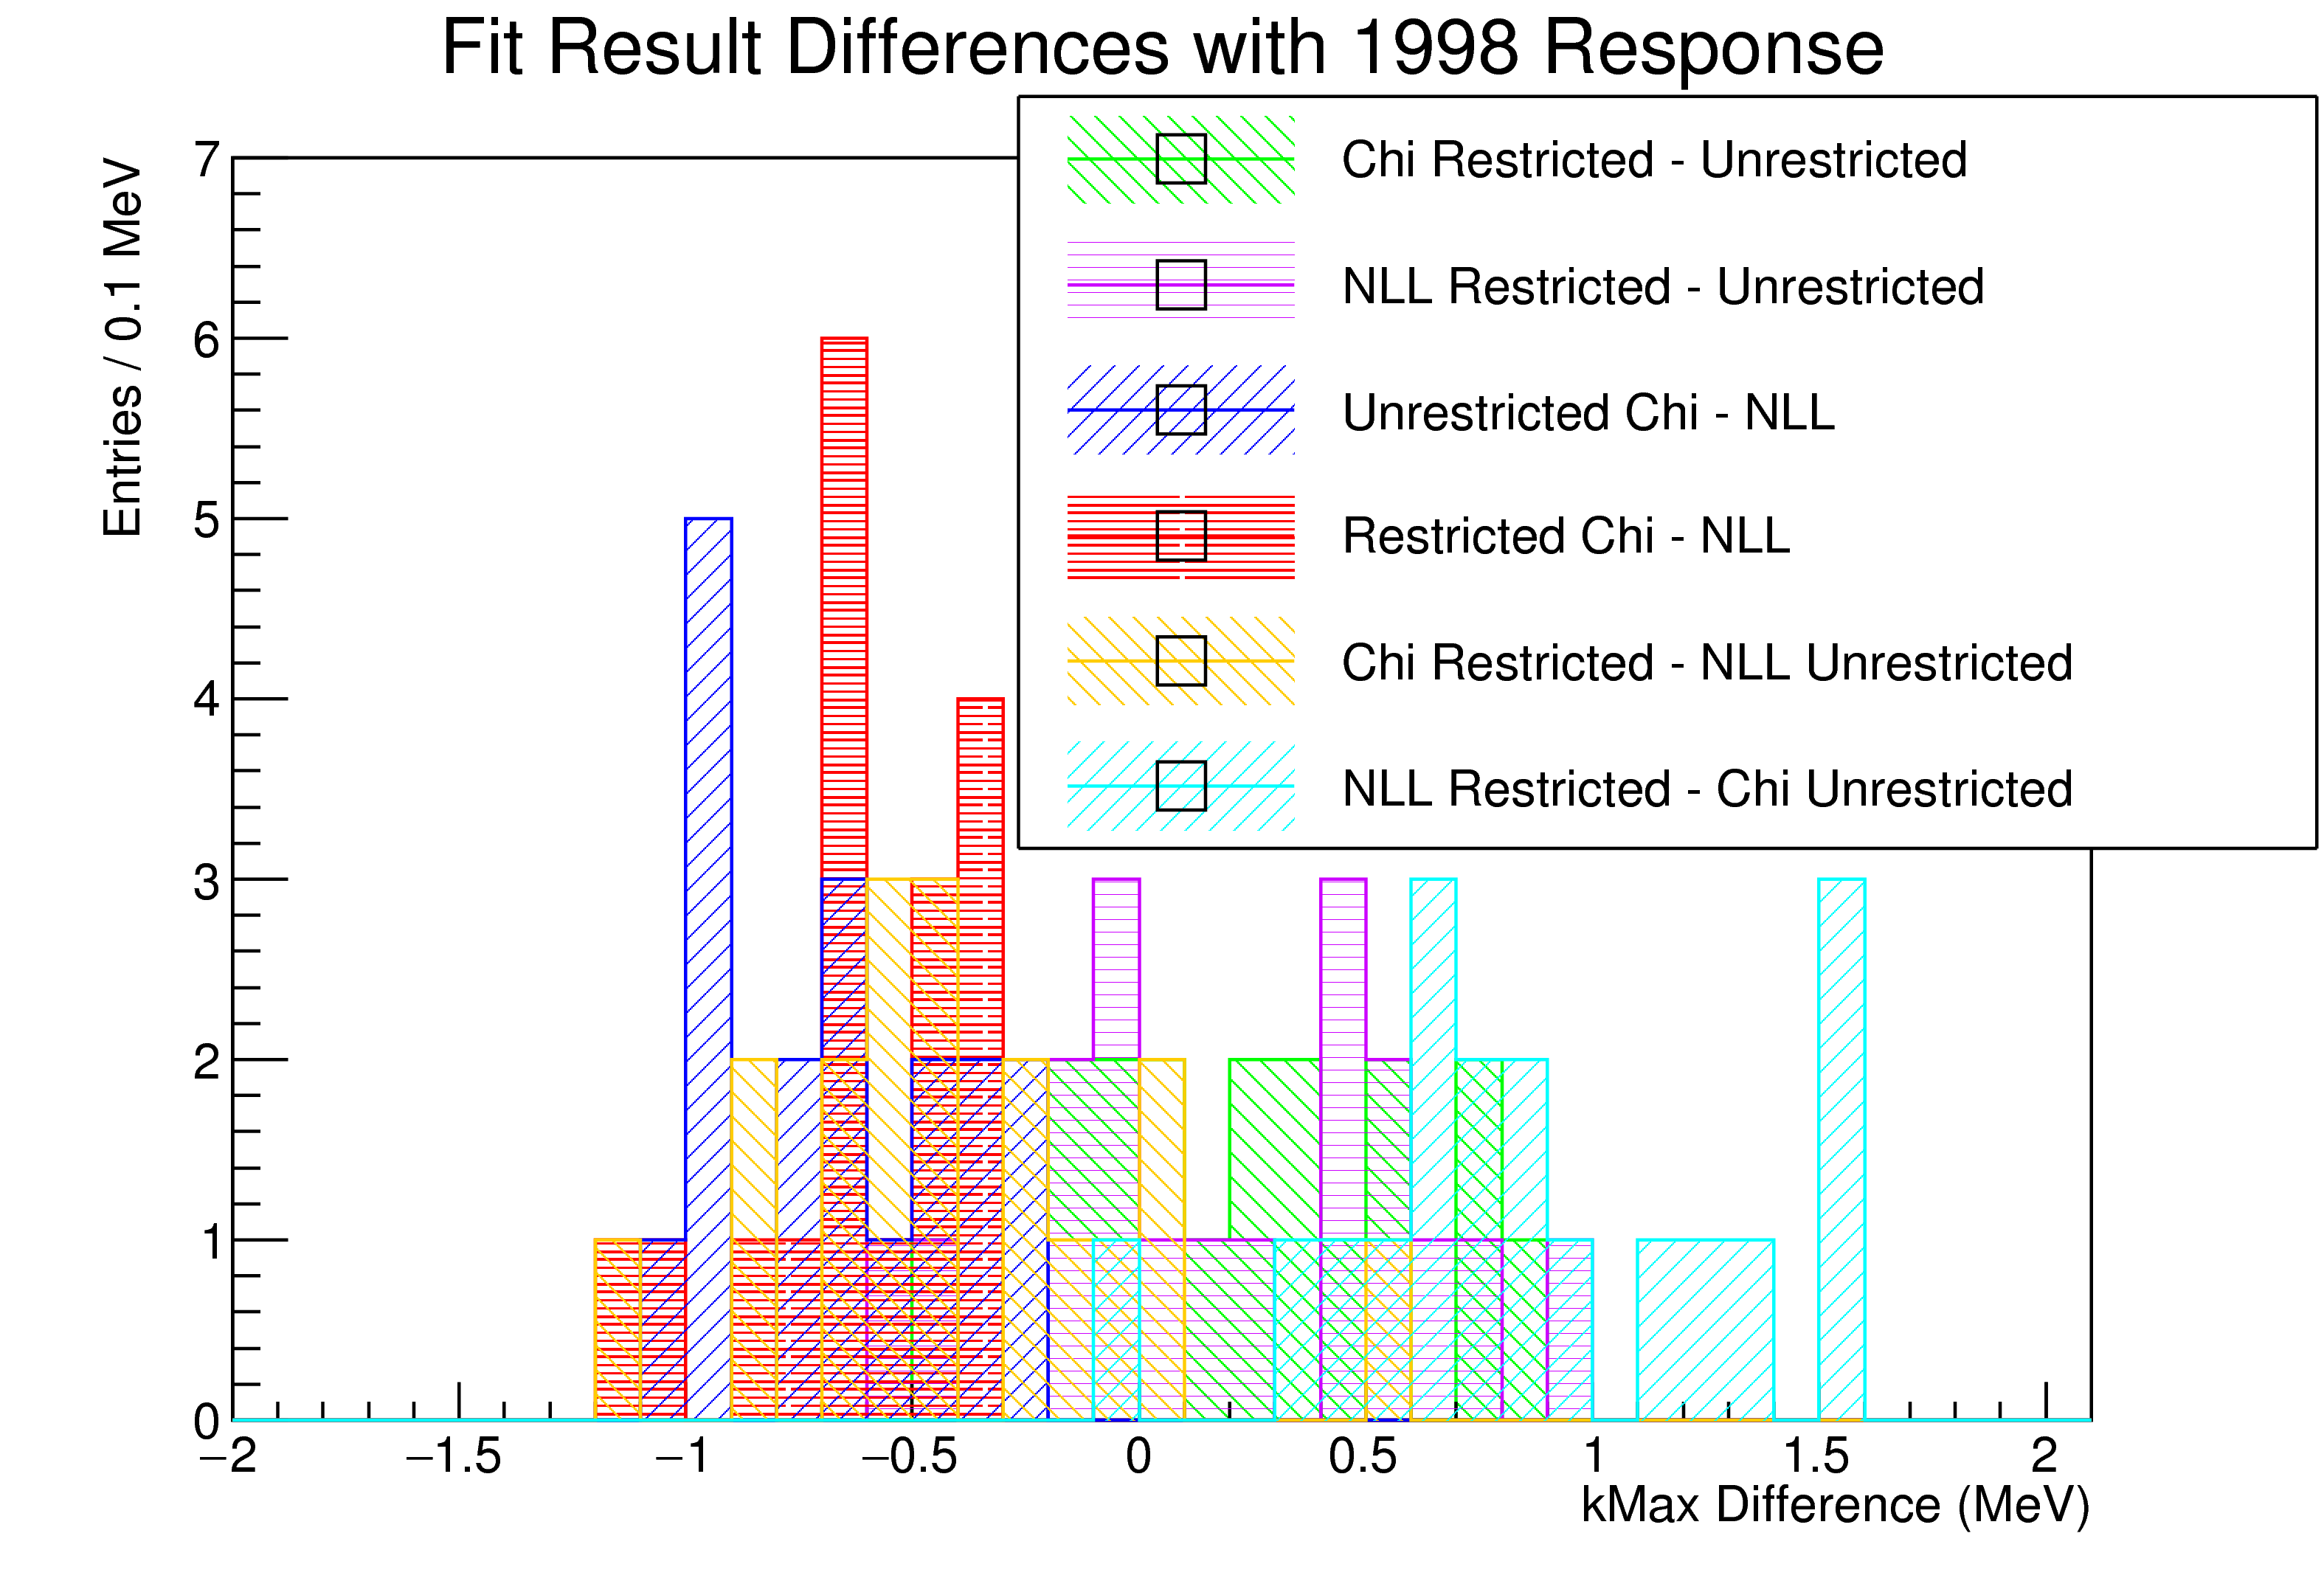
\includegraphics[width=\linewidth]{figures/png/compare_fit_results.png}
  \caption{Plot of the difference between the end point values found using $\chi^2$ and
    NLL minimization with and without a restricted range using the 1998 response function.}
  \label{fig:compareFits}
\end{figure}

\begin{figure}[h]
  \centering
  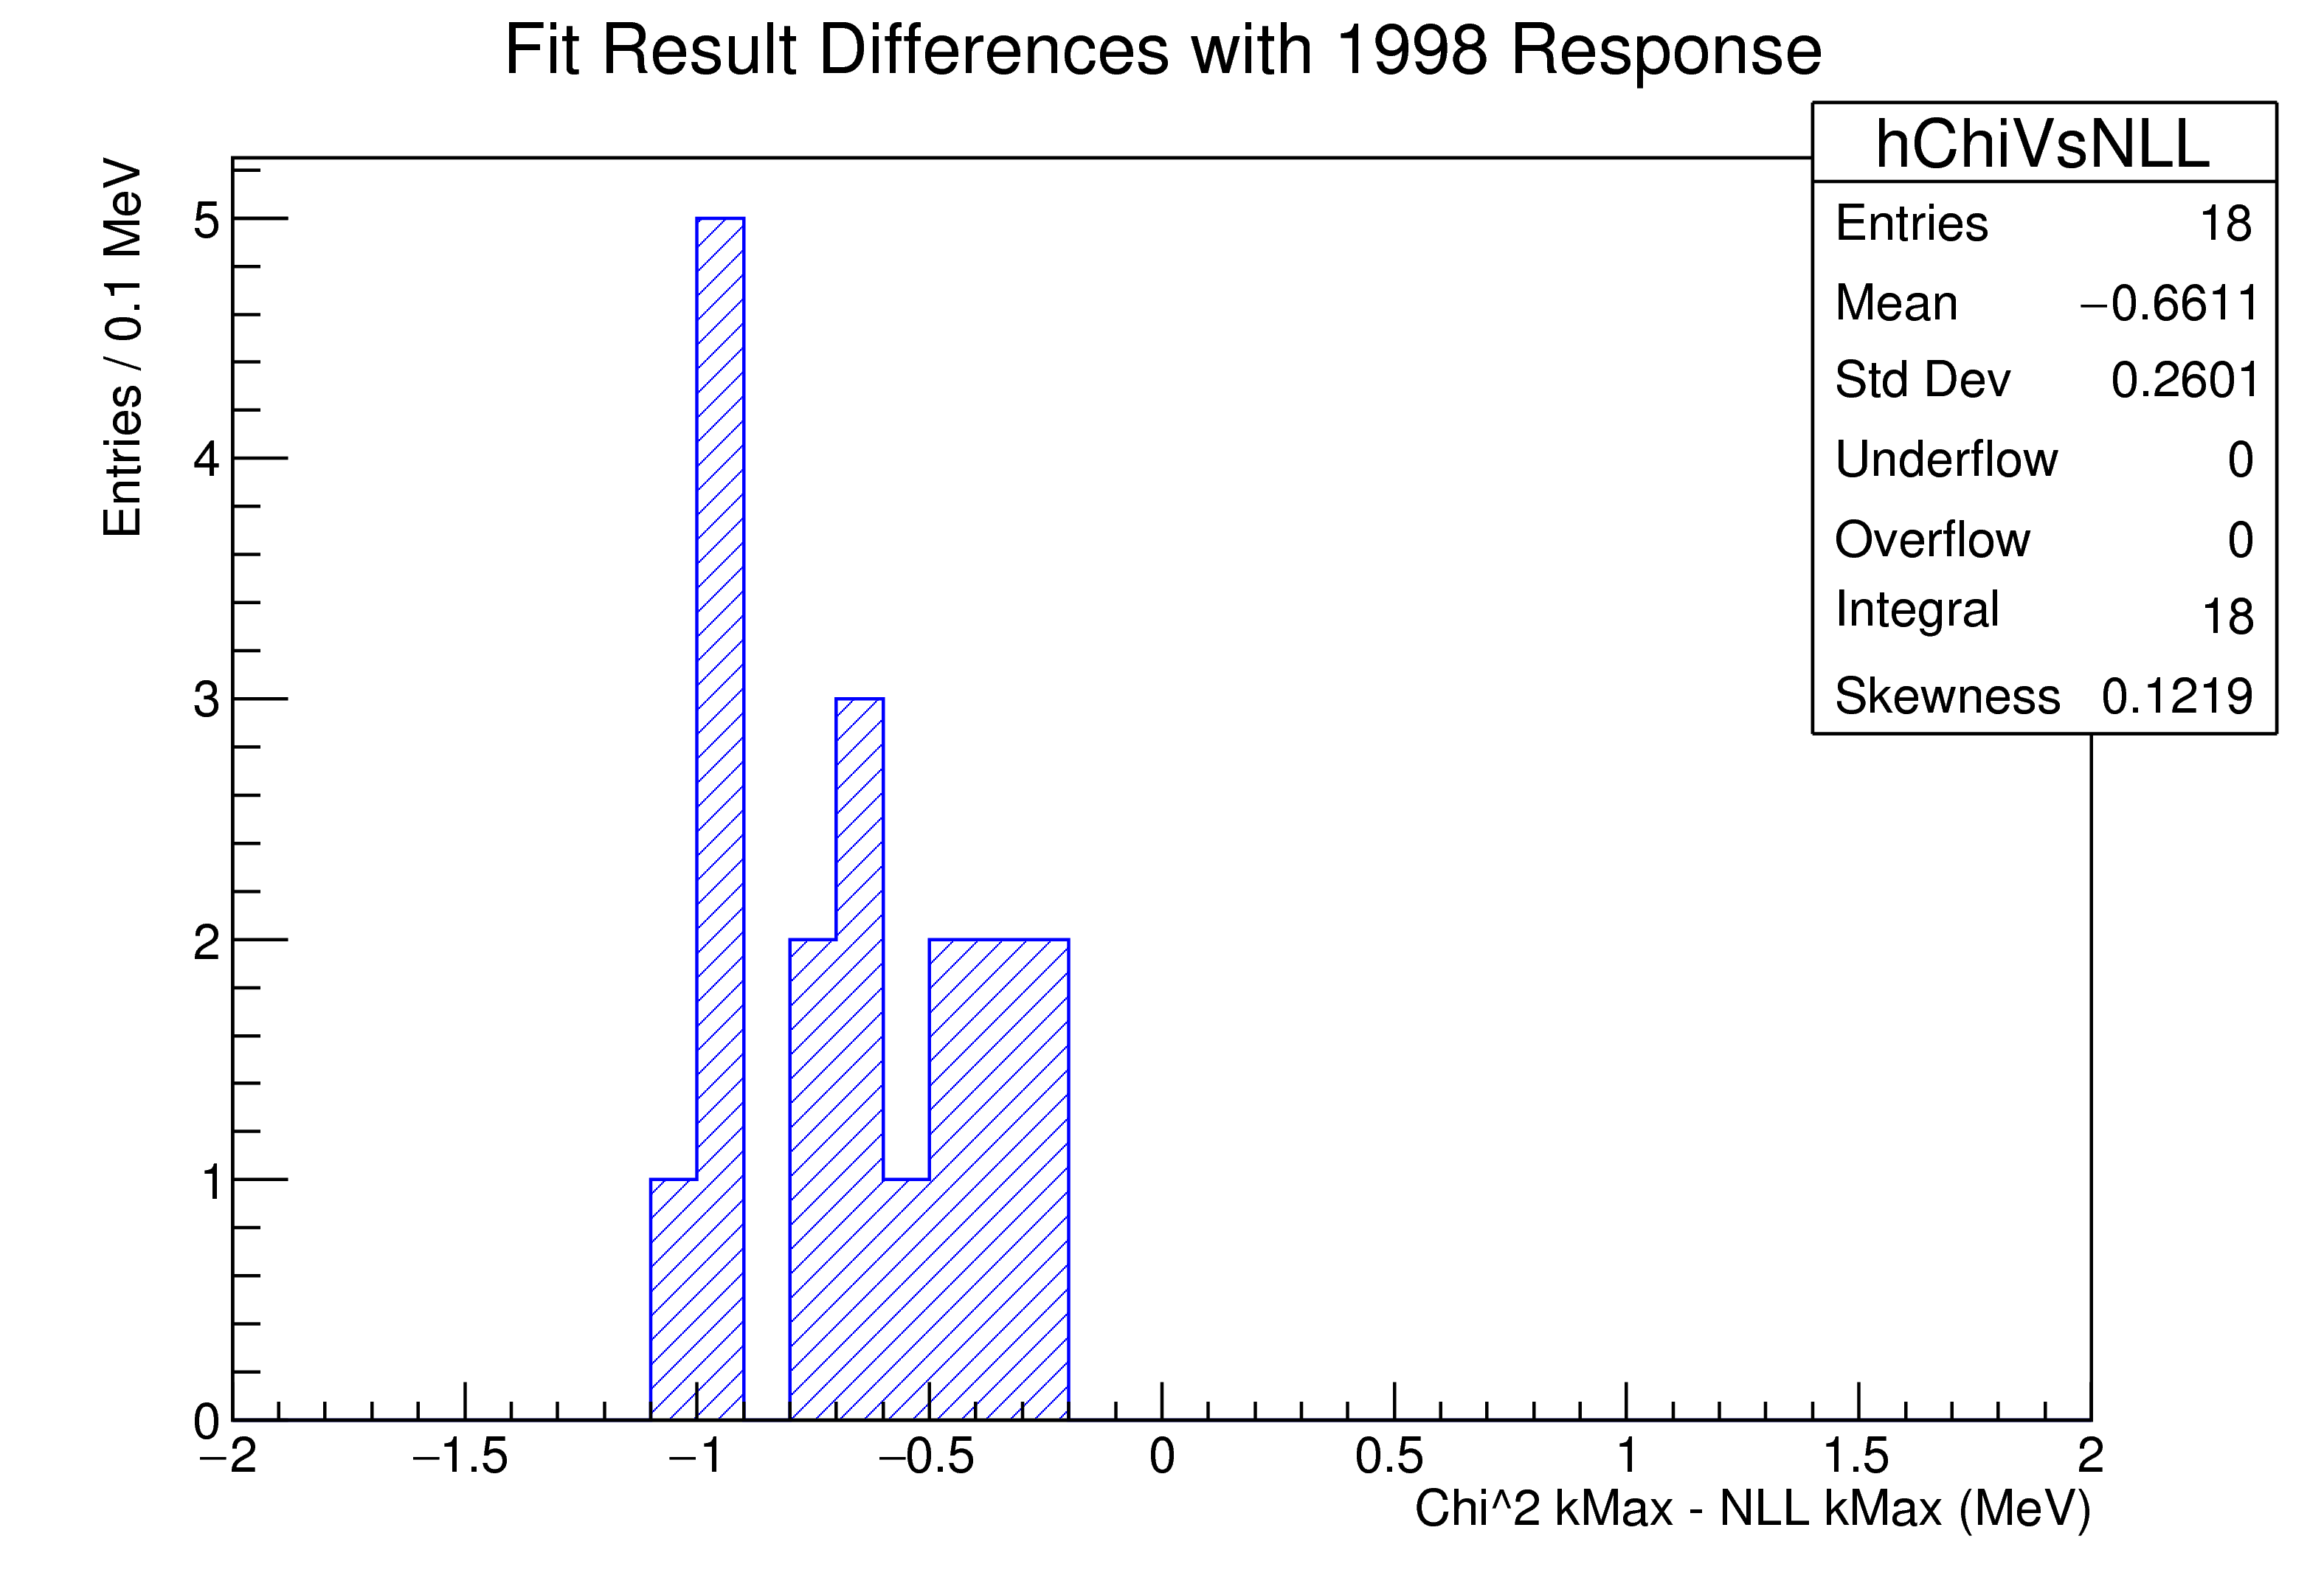
\includegraphics[width=\linewidth]{figures/png/compare_fit_results_unrestrictedOnly.png}
  \caption{Plot of the difference between the end point values found using $\chi^2$ and
    NLL minimization using the 1998 response function.}
  \label{fig:compareFits}
\end{figure}


%% Restricted Range Results (cut top 0.5% and below 60 MeV):
%% Year, Response, Target, kMax, kErr, chi: 1991 1992 Ca Chi 92.66 0.52 chi 3.6 NLL 94.99 0.32 chi 4.3 
%% Year, Response, Target, kMax, kErr, chi: 1992 1992 Al Chi 88.68 0.50 chi 1.6 NLL 90.30 0.37 chi 2.1 
%% Year, Response, Target, kMax, kErr, chi: 1992 1992 Si Chi 89.99 0.43 chi 2.9 NLL 91.62 0.28 chi 3.3 
%% Year, Response, Target, kMax, kErr, chi: 1992 1992 Ca Chi 91.66 0.40 chi 2.8 NLL 94.00 0.28 chi 4.2
%% Year, Response, Target, kMax, kErr, chi: 1992 1992 Mo Chi 88.67 0.47 chi 1.6 NLL 89.63 0.32 chi 1.7
%% Year, Response, Target, kMax, kErr, chi: 1992 1992 Sn Chi 86.70 0.54 chi 2.1 NLL 88.08 0.34 chi 2.2
%% Year, Response, Target, kMax, kErr, chi: 1992 1992 Pb Chi 83.17 0.53 chi 1.3 NLL 85.07 0.38 chi 1.8
%% Year, Response, Target, kMax, kErr, chi: 1995 1992 Al Chi 85.93 0.34 chi 2.3 NLL 87.03 0.23 chi 2.7
%% Year, Response, Target, kMax, kErr, chi: 1995 1992 Si Chi 85.58 0.29 chi 4.0 NLL 86.83 0.23 chi 4.5
%% Year, Response, Target, kMax, kErr, chi: 1995 1992 Ti Chi 85.89 0.48 chi 3.3 NLL 87.29 0.31 chi 3.6
%% Year, Response, Target, kMax, kErr, chi: 1995 1992 O Chi 84.31 0.37 chi 3.3 NLL 85.14 0.25 chi 3.4
%% Year, Response, Target, kMax, kErr, chi: 1995 1992 Ag Chi 85.53 0.67 chi 1.3 NLL 87.23 0.48 chi 1.5
%% Year, Response, Target, kMax, kErr, chi: 1995 1992 Zr Chi 86.04 0.59 chi 1.9 NLL 87.22 0.43 chi 2.0
%% Year, Response, Target, kMax, kErr, chi: 1998 1992 Ni58 Chi 88.46 0.58 chi 1.7 NLL 89.96 0.40 chi 2.0
%% Year, Response, Target, kMax, kErr, chi: 1998 1992 Ni60 Chi 86.31 0.45 chi 2.5 NLL 88.19 0.34 chi 3.2
%% Year, Response, Target, kMax, kErr, chi: 1998 1992 Ni62 Chi 85.41 0.64 chi 1.5 NLL 87.32 0.43 chi 1.7
%% Year, Response, Target, kMax, kErr, chi: 1999 1992 Ti Chi 87.18 0.48 chi 3.6 NLL 88.73 0.31 chi 3.8
%% Year, Response, Target, kMax, kErr, chi: 1999 1992 O Chi 86.15 0.38 chi 3.8 NLL 87.08 0.24 chi 3.7
%% Year, Response, Target, kMax, kErr, chi: 1991 1998 Ca Chi 93.53 0.49 chi 1.5 NLL 94.18 0.46 chi 1.5
%% Year, Response, Target, kMax, kErr, chi: 1992 1998 Al Chi 89.46 0.54 chi 0.8 NLL 89.78 0.51 chi 1.3
%% Year, Response, Target, kMax, kErr, chi: 1992 1998 Si Chi 90.78 0.44 chi 1.3 NLL 91.46 0.43 chi 1.4
%% Year, Response, Target, kMax, kErr, chi: 1992 1998 Ca Chi 93.03 0.42 chi 1.4 NLL 93.50 0.41 chi 1.7
%% Year, Response, Target, kMax, kErr, chi: 1992 1998 Mo Chi 89.06 0.49 chi 0.8 NLL 89.56 0.48 chi 0.8
%% Year, Response, Target, kMax, kErr, chi: 1992 1998 Sn Chi 87.38 0.58 chi 0.7 NLL 87.71 0.53 chi 0.7
%% Year, Response, Target, kMax, kErr, chi: 1992 1998 Pb Chi 83.37 0.54 chi 0.6 NLL 84.07 0.50 chi 0.6
%% Year, Response, Target, kMax, kErr, chi: 1995 1998 Al Chi 85.87 0.33 chi 1.1 NLL 86.64 0.34 chi 0.6
%% Year, Response, Target, kMax, kErr, chi: 1995 1998 Si Chi 85.89 0.35 chi 2.8 NLL 86.90 0.35 chi 3.0
%% Year, Response, Target, kMax, kErr, chi: 1995 1998 Ti Chi 86.11 0.48 chi 1.6 NLL 86.51 0.42 chi 1.6
%% Year, Response, Target, kMax, kErr, chi: 1995 1998 O Chi 84.51 0.40 chi 1.5 NLL 85.12 0.38 chi 1.1
%% Year, Response, Target, kMax, kErr, chi: 1995 1998 Ag Chi 85.91 0.71 chi 0.7 NLL 86.58 0.66 chi 0.8
%% Year, Response, Target, kMax, kErr, chi: 1995 1998 Zr Chi 85.89 0.65 chi 1.4 NLL 86.53 0.58 chi 1.5
%% Year, Response, Target, kMax, kErr, chi: 1998 1998 Ni58 Chi 88.63 0.61 chi 1.1 NLL 89.77 0.62 chi 1.3
%% Year, Response, Target, kMax, kErr, chi: 1998 1998 Ni60 Chi 86.93 0.51 chi 1.3 NLL 87.52 0.46 chi 1.3
%% Year, Response, Target, kMax, kErr, chi: 1998 1998 Ni62 Chi 85.89 0.64 chi 0.8 NLL 86.71 0.63 chi 0.8
%% Year, Response, Target, kMax, kErr, chi: 1999 1998 Ti Chi 87.69 0.48 chi 1.6 NLL 88.08 0.42 chi 1.4
%% Year, Response, Target, kMax, kErr, chi: 1999 1998 O Chi 86.71 0.41 chi 1.5 NLL 87.10 0.37 chi 1.3

